\documentclass[conference]{IEEEtran}
\IEEEoverridecommandlockouts
% The preceding line is only needed to identify funding in the first footnote. If that is unneeded, please comment it out.
%Template version as of 6/27/2024

\usepackage{cite}
\usepackage{amsmath,amssymb,amsfonts}

\usepackage{latexsym}
\usepackage{caption,booktabs,amsthm,amsmath,threeparttable,subfigure,float}
% \usepackage{algorithmic}
\usepackage{graphicx}
\usepackage{textcomp}
\usepackage{xcolor}
% \usepackage[ruled,linesnumbered]{algorithm2e}
\usepackage{algorithm,algorithmic}


\def\BibTeX{{\rm B\kern-.05em{\sc i\kern-.025em b}\kern-.08em
    T\kern-.1667em\lower.7ex\hbox{E}\kern-.125emX}}
\begin{document}

    \title
    {
        Asymptotically time-optimal smooth trajectory planning in dynamic environments\\
    }

    \author
    {
        \IEEEauthorblockN{Hang Zhou}
        \IEEEauthorblockA{\textit{School of Aeronautics and Astronautics} \\
        \textit{Zhejiang University}\\
        Hangzhou, China \\
        zhou\_hang@zju.edu.cn}
        \and
        \IEEEauthorblockN{Tao Meng}
        \IEEEauthorblockA{\textit{School of Aeronautics and Astronautics} \\
        \textit{Zhejiang University}\\
        Hangzhou, China \\
        mengtao@zju.edu.cn}
    }

    \maketitle

    \begin{abstract}
        In this paper we proposed an algorithm for smooth trajectory generation in complex environments with dynamic obstacles and velocity constraints. The proposed algorithm Tube Space-Time RRT* (TubeST-RRT*) is combined with the improved reformulation dynamic coordinate minimum snap (RDCMS) to generate smooth collision-free trajectories with asymptotic time Optimal.First, sample the space-time state space to obtain the time information for each node to complete the avoidance of moving obstacles.Then, to address the issue of non-smooth paths in ST-RRT*, generate a dynamic Tube for each node and combine it with the improved minisnap to create a smooth, collision-free trajectory Finally,Simulations in complex environments demonstrate the effectiveness of our proposed algorithm.
    \end{abstract}

    \begin{IEEEkeywords}
        Tube Space-Time RRT*; asymptotic time Optimal; smooth collision-free trajectories
    \end{IEEEkeywords}

    \section{Introduction}
        Trajectory planning is a fundamental challenge in robotics\cite{b1}, as obstacles in the real world often change over time. Applications such as robotics and autonomous driving typically require a smooth, collision-free trajectory. Assuming the obstacle trajectories are known a priori, the problem can be modeled as navigation in a dynamic environment. Mathematically, this is expressed as planning through a space-time state space \cite{b2}.

        Planning in dynamic environments has been studied for a long time and has yielded significant research results. These results can be broadly categorized into two approaches. For example, RRTX\cite{b3} and Real-time RRT* \cite{b4} require fast replanning when previously computed paths become invalid during execution. However, as the dimensionality increases, the replanning time becomes longer, making it difficult to respond to moving obstacles. Risk-RRT \cite{b5} combines predictions of obstacle movements and computes partial motion paths to keep the collision probability below a given threshold. However, since only partial paths are returned, frequent replanning is still necessary.Another approach assumes that the trajectories of moving obstacles are unknown, while another assumes that the trajectories of the obstacles are completely known. For example, Time-Based RRT \cite{b6} extends the configuration state space through the time dimension and unidirectionally plans to a set of known target states. However, it requires the assumption of knowing the specific time for each target configuration. Additionally, due to the random sampling nature of RRT, the resulting trajectories are usually not smooth.

        In this paper, we proposes a Tube-based space-time sampling planning algorithm, TubeST-RRT*, and an improved reformulation dynamic coordinate minimum snap (RDCMS) method. Through a two-step method of  planning and optimizing, it achieves asymptotic time-optimal collision-free trajectory planning in dynamic environments, while ensuring high trajectory smoothness to facilitate easier tracking control. The TubeST-RRT* algorithm adds a time dimension to the configuration space so that each node contains time information, allowing it to respond to time-varying obstacles. Additionally, the improved RDCMS method combines with each node's tube information and time information to generate smooth, collision-free trajectories. Finally, comparative simulations verify the effectiveness of the algorithm

        The rest of this paper is organized as follows: At Section \ref{sec2}, explains the problem of time-optimal planning in dynamic environments. In Section III,presents the main results of this paper, including the principles and steps of the Tube ST-RRT* planning algorithm and the RDCMS trajectory optimization algorithm. Section IV provides simulation results and comparative experiments to demonstrate the feasibility and superiority of the proposed method. Finally, Section V summarizes the paper.
    \section{Problem Statement}
    \label{sec2}
    Consider the time-space planning problem with a tube, where the space-time state space is defined as \(\mathcal{Q} = \mathcal{X} \times \mathcal{T} \times \mathcal{B}\), where \(\mathcal{X} \subset \mathbb{R}^n\) is the configuration state space, \(\mathcal{T}\) is the time state space, \(\mathcal{B}\) is the size of the tube, and \(n\) is the dimension of the configuration space state. Let \(\mathcal{Q}_{free} \subset \mathcal{Q}\) be the collision-free subset of states, \(Q_{start}\) be the initial state, and \(\mathcal{X}_{goal}\) be the goal region. In the following work, it is assumed that the trajectories of obstacles are completely known. Therefore, the planning problem can be described as finding a path solution that starts from the initial state \(q_{start}\), reaches the goal region or target state \(x_{goal} \in \mathcal{X}_{goal}\). The goal is to find a state-space sequence with the tube size as large as possible and the time taken as short as possible while avoiding time-varying obstacles.

    % \begin{equation}
    % \begin{aligned}
    %     \label{problem}
    %     &\min \quad \int_{t_{start}}^{t_{goal}}1dt \\
    %     &s.t. \quad x(t_{init}) = x_{init} \\
    %     &\dot{\boldsymbol{x}}(t) = \boldsymbol{A}\boldsymbol{x}+\boldsymbol{B}\boldsymbol{u}\\
    %     & \boldsymbol{x}(t) \in \mathcal{X}_{free},t \in [t_{init},t_{final}]
    % \end{aligned}
    % \end{equation}

    \section{Main Results}
    \label{sec3}
    \subsection{Path Node Generation Based on TubeST-RRT*}
    % TubeST-RRT* 算法是 RRT* Connect 算法的增强版本,对采样函数、引导函数、最近邻函数和重连函数进行了修改。由于节点具有时间信息,可以引入运动检查函数进行速度约束的检测,此外,在状态空间中添加了额外的tube维度以保证采样节点与障碍物的最小距离。通过考虑障碍物的时间变化特性和添加节点的tube,该算法确保生成的轨迹在后续的轨迹优化过程中保持安全且无碰撞。
    The TubeST-RRT* algorithm is an enhanced version of the RRT* Connect \cite{b7} algorithm , with modifications to the sampling function, steering function, nearest neighbor function, and rewiring function. Since the nodes contain time information, a motion check function can be introduced to detect velocity constraints. Additionally, an extra tube dimension is added to the state space to ensure a minimum distance between sampling nodes and obstacles. By considering the time-varying characteristics of obstacles and incorporating the tube into the nodes, the algorithm ensures that the generated trajectory remains safe and collision-free throughout subsequent trajectory optimization.
    
    % RRT* Connect 算法是一种渐进最优的双向采样方法,广泛应用于具有避障约束的机器人路径规划中。RRT 方法的核心思想是在状态空间中随机采样,以获取从父节点到子节点的一系列路径节点和有向边,形成搜索树 $\mathcal{T}_{tree }$。为了在具有时变障碍物的环境中解决规划问题,提出了 Tube-ST-RRT* 算法。该算法首先在状态空间中添加一个时间维度,并对节点时间进行采样,以获得满足时变约束的节点。其次,在节点采样过程中,采样tube变量以确保节点在该半径的球形区域内无碰撞。最终结果是节点序列 $\boldsymbol{s} = [\boldsymbol{s_{0}},\boldsymbol{s}_{1}\dots{},\boldsymbol{s}_{n}]$,其中每个节点都包含位置信息、速度、时间以及最大无碰撞球形区域的半径信息。
    RRT* Connect algorithm is an asymptotically optimal bidirectional sampling method widely used in robot path planning with obstacle avoidance constraints. The core idea of the RRT method is to randomly sample in the state space to obtain a series of path nodes and directed edges from the parent node to the child node, forming a search tree ${T}_{tree }$. To address planning problems in environments with time-varying obstacles, the TubeST-RRT* algorithm is proposed. This algorithm first adds a time dimension to the state space and samples the node times to obtain nodes that meet the time-varying constraints. Secondly, during the node sampling process, a tube variable is sampled to ensure that the node is collision-free within a spherical region of that radius. The final result is a sequence of nodes $\boldsymbol{s} = [\boldsymbol{s_{0}},\boldsymbol{s}_{1}\dots{},\boldsymbol{s}_{n}]$, each containing information on position, velocity, time, and the radius of the maximum collision-free spherical region. 

    % Tube-ST-RRT* 算法的详细步骤见算法 \ref{algorrt}。算法输入除了 $\mathcal{S}$、$q_{start}$、$\mathcal{X}_{goal}$ 和 $d$ 外,还需要规划终止条件 $ptc$、采样新目标的概率 $p_{goal} \in \left (0, 1 \right ]$ 以及时间限制 $t_{\max} \in \left (0, \infty \right]$。基本框架与 RRT-Connect 类似。
    The algorithmic details of TubeST-RRT* are provided in Algorithms \ref{algorrt}. The algorithm inputs, in addition to $\mathcal{Q}, q_{start}, \mathcal{X}{goal}, d$, the planning termination condition $ptc$, the probability of sampling a new goal $p_{goal} \in \left (0, 1 \right ]$, and the time limit $t_{\max} \in  (0, \infty ]$ are also required. The basic framework is similar to RRT-Connect. 

    Algorithm \ref{algorrt} outlines the overall framework of TubeST-RRT*. The general procedure of the algorithm is as follows:

    % “首先,算法寻找起点的最小无碰撞半径 $r_{init}$,然后初始化参数。在每次迭代中,首先更新边界参数。接着,以概率 $p_{goal}$ 决定是否采样一个新目标或采样终点以得到采样点$q_{rand}$。然后找到离采样点的最近点 $q_{near}$,并在 $q_{near}$ 和 $q_{rand}$ 之间扩展得到 $q_{new}$。在 $q_{new}$ 中,找到最大无碰撞球形的半径R。如果从 $q_{near}$ 到 $q_{new}$ 的路径无碰撞且满足速度约束,则将新状态 $q_{new}$ 添加到当前树 $T_{a}$ 中,并尝试从 $q_{new}$ 连接到另一棵树 $T_{b}$。如果连接成功,则更新解决方案。最后,交换 $T_{a}$ 和 $T_{b}$,并开始下一次迭代。重复直到满足终止条件 $ptc$。”
    First, the algorithm finds the minimum collision-free radius \( r_{init} \) for the starting point and initializes the parameters. In each iteration, boundary parameters are updated. Then, with a probability \( p_{goal} \), it decides whether to sample a new goal or sample the endpoint to obtain the sampling point \( q_{rand} \). Next, it finds the nearest point \( q_{near} \) to the sampling point and extends between \( q_{near} \) and \( q_{rand} \) to obtain \( q_{new} \). At \( q_{new} \), the maximum collision-free spherical radius \( R \) is determined. If the path from \( q_{near} \) to \( q_{new} \) is collision-free and satisfies the velocity constraints, the new state \( q_{new} \) is added to the current tree \( T_{a} \), and an attempt is made to connect \( q_{new} \) to the other tree \( T_{b} \). If the connection is successful, the solution is updated. Finally, \( T_{a} \) and \( T_{b} \) are swapped, and the next iteration begins. This process is repeated until the termination condition \( ptc \) is met.

    % 蓝色区域表示动态障碍物,随时间变化从左边移动到右边,橙色圆表示当前节点生成的最大无碰撞圆,算法最终生成一条每个节点具有无碰撞圆的路径,保证了无碰撞同时也为后续的轨迹优化提供了基础
    As Fig.(\ref{fig2}) shows,the blue area represents dynamic obstacles, which move from left to right over time. The orange circle indicates the maximum collision-free circle generated at the current node. The algorithm ultimately generates a path where each node has a collision-free circle, ensuring collision avoidance and providing a foundation for subsequent trajectory optimization.
    \begin{figure}
		\centering
		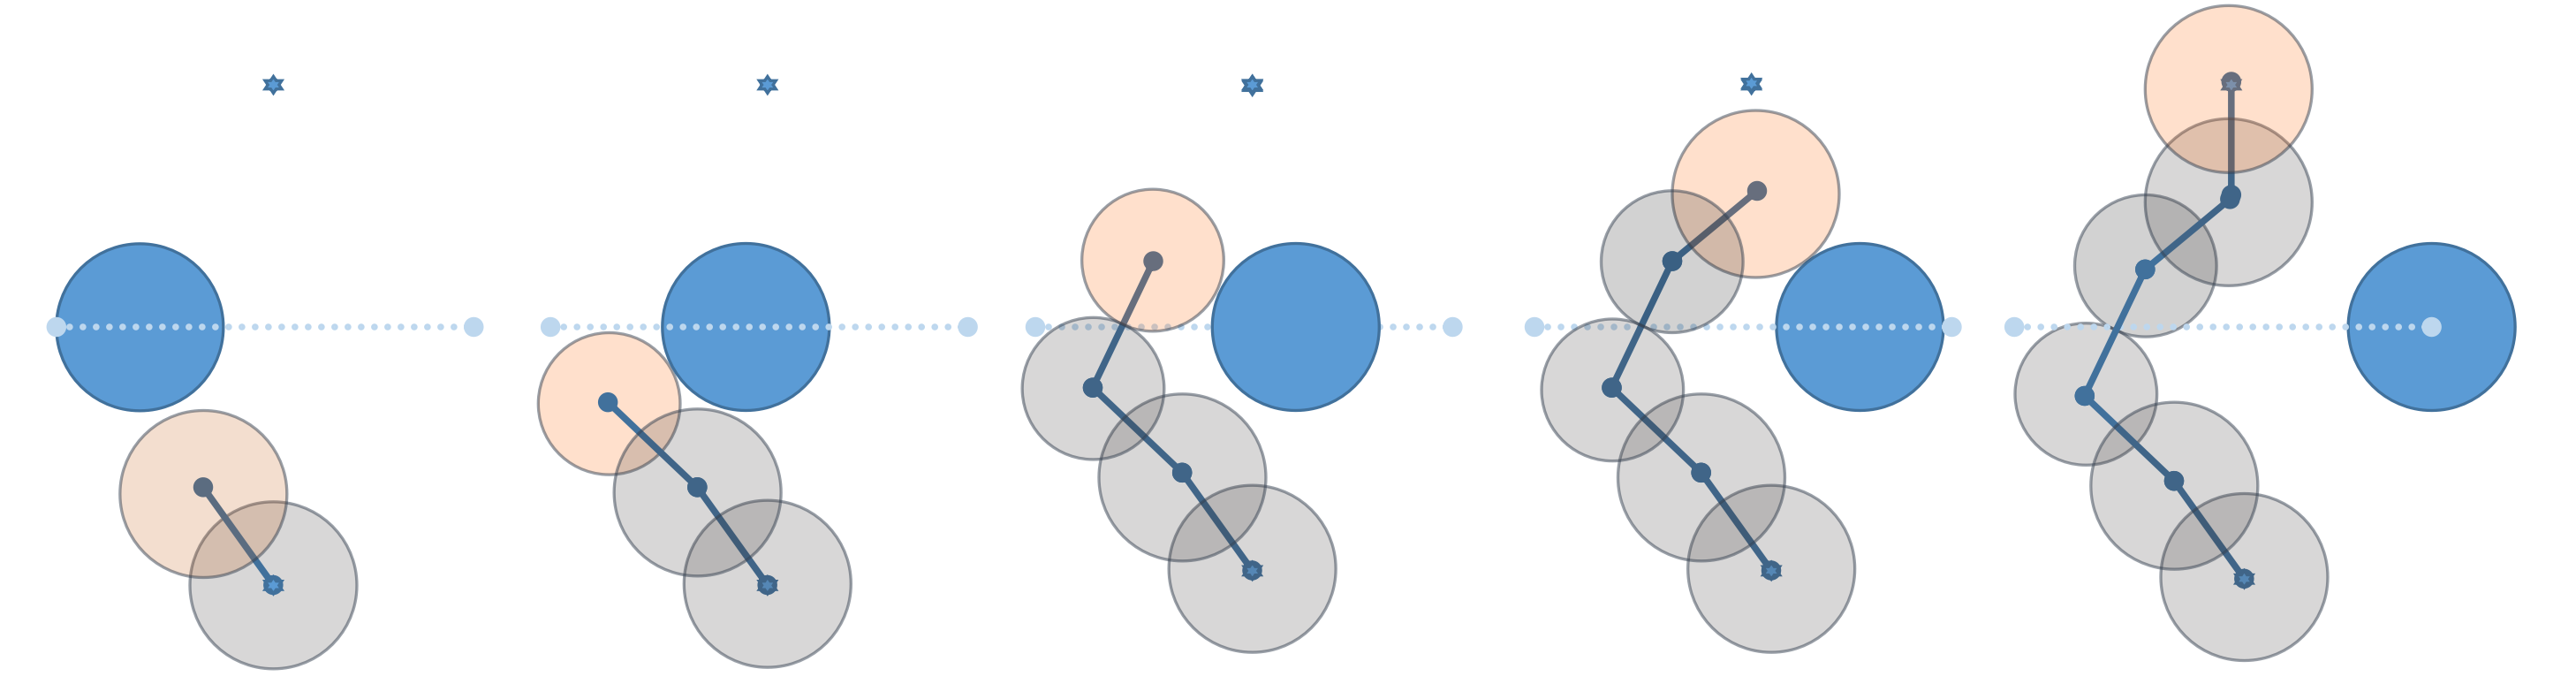
\includegraphics[scale=0.07]{fig2.png}
		\caption{llustration of the Expansion Method in TubeST-RRT}
		\label{fig2}
	\end{figure}

    The main improvements of our proposed TubeST-RRT* algorithm over RRT*-Connect are as follows:
    \begin{itemize}
        % Tube-ST-RRT* 生成一系列具有半径 $R_i$ 和时间信息的相交球,如图 b 所示。则所有球的内部会结合会形成一个无碰撞的飞行走廊,确保了由 minisnap 生成的轨迹是无碰撞的。
        \item TubeST-RRT* generates a series of intersecting spheres with radius \(R_i\) with time information, The interior of all the spheres combines to form a collision-free flight corridor, ensuring that the trajectory generated by minisnap is collision-free.
        % 改进的条件采样。任何可能成为解决路径一部分的状态,必须与起点有一个有限距离 \(d\),并且至少与一个目标状态有接触。由于速度限制,只有起始速度区域和目标速度区域的交集中的状态才满足这个要求。因此,与 Informed RRT\* 类似,我们只从可以生成解决方案的区域进行采样。理想情况下,采样应直接从起始速度区域和目标速度区域的并集中进行。
        \item Improved Conditional Sampling. Any state that can be part of the solution path must have a finite distance \(d\) from the starting point and must be in contact with at least one target state. Due to velocity constraints, only states within the intersection of the start velocity region and the target velocity region satisfy this requirement shows in Fig.(\ref{fig_union}). Therefore, similar to Informed RRT*, we sample only from the region where solutions can be generated. Ideally, sampling should occur directly from the union of the start velocity region and the target velocity region.
    \end{itemize}

    \begin{figure}
		\centering
		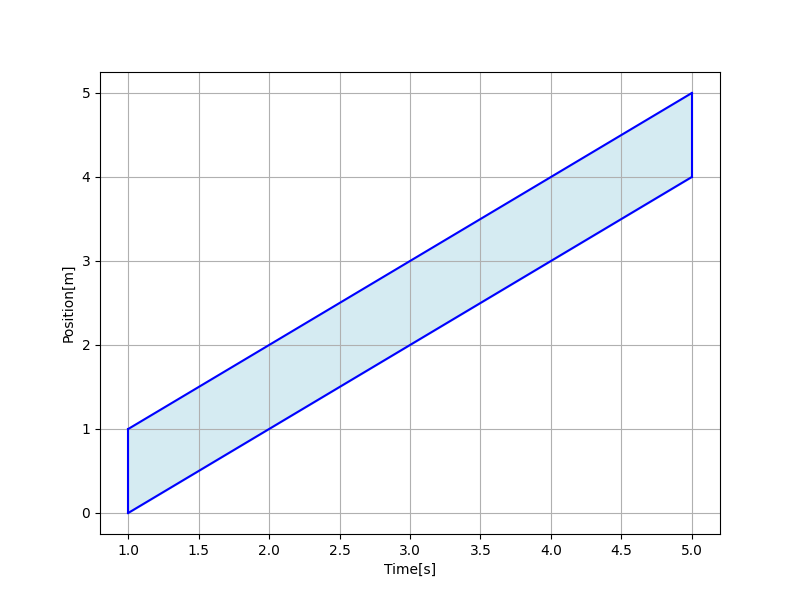
\includegraphics[scale=0.4]{union of the start velocity cone and the target velocity cone.png}
		\caption{union of the start velocity cone and the target velocity cone}
		\label{fig_union}
	\end{figure}
    
    \begin{algorithm}
        \renewcommand{\algorithmicrequire}{\textbf{Input:}}
		\renewcommand{\algorithmicensure}{\textbf{Output:}}
		\caption{TubeST-RRT*}
		\label{algorrt}
        \begin{algorithmic}
            \REQUIRE $\mathcal{Q},q_{start},x_{goal},p_{goal},range\_d,Param,ptc$
            \ENSURE $Soulution$
            \STATE{$r_{start} \gets FindMaxRadius(s_{start})$}
		\STATE{$s_{start} \gets \{q_{start},r_{start}\}$}
		\STATE{$T_{a} \gets \{s_{start}\};T_{b} \gets \emptyset$}
		\STATE{$B \gets InitailieBoundVariables(Param)$}
		\WHILE{ptc}
            \STATE{$B \gets UpdateGoalRegion(B,Param,t_{\max})$}
            \IF{$ p_{goal} > rand(0,1)$}
                \STATE{$B \gets SampleGoal(s_{start},x_{goal},T_{gaol},B)$}
            \ENDIF{}
            \STATE{$q_{rand} \gets SampleConditionally(s_{start},\mathcal{Q},B, d)$}
            \STATE{$r_{rand} \gets FindMaxRadius (q_{rand})$}
            \STATE{$s_{rand} \gets \{q_{rand},r_{rand}\}$}
            \STATE{$s_{nearsst} \gets Nearset(s_{rand},T_{a})$}
            \STATE{$s_{new} \gets TubeSTSteer(s_{nearest},s_{rand},d)$}
            \IF{$MotionCheck(s_{nearsst},s_{new})$}
                \STATE{${Rewire}Tree(T_{a},x_{new})$}
                \IF{$Connect(T_{b}, x_{new}, d) = Reached$}
                    \STATE{$solution \gets UpdateSolution(x_{new})$}
                    \STATE{$t_{\max} \gets CostPath(solution)$}
                    \STATE{$PruneTrees(t_{\max}, T_a, T_b)$}
                \ENDIF{}
            \ENDIF{}
            \STATE{$Swap(T_a,T_b)$}
		\ENDWHILE{}
		\RETURN{$Solution$}
        \end{algorithmic}
    \end{algorithm}

    \subsection{Reformulation Dynamic Coordinate Minimum Snap Trajectory Optimization}
    % 对于由 TubeST-RRT\* 生成的状态序列,我们使用提出的RDCMS轨迹优化来使轨迹平滑。在最小快照轨迹优化中,优化后的轨迹需要通过中间路径节点。然而,由于我们的 TubeST-RRT\* 在球形区域内集成了碰撞检测,它提供了一个无碰撞的飞行走廊。因此,轨迹只需要保持在这个走廊内即可确保无碰撞运动。传统的使用多项式参数作为优化变量的最小快照优化可能在节点过多时导致数值不稳定。在这里,我们可以使用重构最小快照,将优化变量从多项式系数转化为物理上有意义的变量,如位置 (\(p\))、速度 (\(v\)) 和加速度 (\(a\))。可以对 \(p\) 添加不等式约束,以确保它保持在规划器生成的tube区域内。这确保了优化后的轨迹是无碰撞的。
    For the state sequences generated by TubeST-RRT*, we use the proposed RDCMS trajectory optimization to smooth the trajectories. In traditional minimum snap trajectory optimization, the optimized trajectory needs to pass through intermediate path nodes. However, since our TubeST-RRT* incorporates collision detection within the spherical regions, it provides a collision-free flight corridor. Therefore, the trajectory only needs to stay within this corridor to ensure collision-free movement. Traditional minimum snap optimization using polynomial parameters as optimization variables may lead to numerical instability when there are too many nodes. Here, we can use reformulation minimum snap to transform the optimization variables from polynomial coefficients to physically meaningful variables such as position ($p$), velocity ($v$), and acceleration ($a$). Inequality constraints can be added to $p$ to ensure it stays within the tube area generated by the planner. This ensures that the optimized trajectory is collision-free.
    Input as
    \begin{equation}
        \boldsymbol{S} = [\boldsymbol{s}_{0},\boldsymbol{s}_{1},\boldsymbol{s}_{2},\cdot{}\cdot{}\cdot{},\boldsymbol{s}_{N}]
    \end{equation}
    where,$\boldsymbol{s}_{i} = [\boldsymbol{p}_{i},\boldsymbol{v}_{i},t_{i},r_{i}]$
    A quintic polynomial is used to fit a uniaxial trajectory.
    \begin{equation}
        \boldsymbol{p}\left( {t}\right)= {p}_{0} {t}^{0}+ {p}_{1} {t}^{1}+\cdots+ {p}_{5} {t}^{5}
    \end{equation}

    For the $N+1$ points generated by the planner (including the start point and the end point), it can be assumed that there are $N$ segments of the trajectory, where each segment of the trajectory is a higher-order polynomial, for RDCMS, our cost function is

    \begin{equation}
        J= J_{1}+J_{2}+\cdots+J_{N} = \sum_{n=0}^M p_{m}^\top Q_{m}p_{m}
    \end{equation}

    where,$J_{m} = \int^{T_{m}}_{{T_{m-1}}}\left( \frac{d^4p(t)}{dt^4} \right)^2$
    However, as the polynomial coefficients do not have practical physical meanings, when N is large, or in some special cases, this optimization problem can easily become numerically unstable, leading to difficulties in solving. To address this issue, a reformulation method was proposed to map the optimization variables to the physically meaningful variables $(p,v,a)$\cite{b8}.
    \begin{equation}
        \begin{aligned}
            \boldsymbol{A}_i\boldsymbol{p}_i=\boldsymbol{d}_i,\quad \boldsymbol{A}_i=\begin{bmatrix}\boldsymbol{A}_0\\\boldsymbol{A}_T\end{bmatrix}_i,\boldsymbol{d}_i=\begin{bmatrix}\boldsymbol{d}_0\\\boldsymbol{d}_T\end{bmatrix}_i
        \end{aligned}
    \end{equation}
    The mapping relationship between the polynomial coefficients and the motion differential has been obtained.
    \begin{equation}
        \begin{aligned}
            & \boldsymbol{d}_{i}
            = 
            \boldsymbol{A}_{i} 
            \boldsymbol{p}_{i} \\
            & \boldsymbol{p}_{i} = \boldsymbol{A}_{i}^{-1}\boldsymbol{d}_{i}
        \end{aligned}
    \end{equation}

    where, $\boldsymbol{d}_{i}$ is a vector including the derivative values of the start $\boldsymbol{d}_0$ and the end $\boldsymbol{d}_T$ of the $i$ segment. If the specific derivative is not known, a continuity constraint needs to be imposed to ensure that the derivative at the end of the $i$ segment matches the derivative at the beginning of the $(i + 1)$ segment: 

    Replace the coefficient vector of the original cost function through the mapping matrix $\boldsymbol{A}_{m}$ to obtain the following equation

    \begin{equation}
        \begin{aligned}
            J 
            &= 
            \begin{bmatrix}\boldsymbol p_0\\\boldsymbol p_1\\\vdots\\\boldsymbol p_ N\end{bmatrix}^\top
            \begin{bmatrix}\boldsymbol Q_0&0&\cdots&\cdots&0\\0&\boldsymbol Q_1&0&\cdots&0\\\vdots&\vdots&\vdots&\ddots&\vdots\\0&0&0&\cdots&\boldsymbol Q_\mathrm N\end{bmatrix}
            \begin{bmatrix}\boldsymbol p_0\\\boldsymbol p_1\\\vdots\\\boldsymbol p_ N\end{bmatrix}
            % \\
            % &= 
            % \begin{bmatrix}
            % \boldsymbol{d}_{0} \\
            % \boldsymbol{d}_{1} \\
            % \vdots  \\
            % \boldsymbol{d}_{N} 
            % \end{bmatrix}^{\top}
            % \begin{bmatrix}
            % \boldsymbol{A} & 0 &\cdots &0 \\
            % 0 & \boldsymbol{A_{1}}  &\cdots &0 \\ 
            % \vdots &\vdots &\ddots &\vdots    \\
            % 0 & 0 &\cdots  &\boldsymbol{A_{N}} \\
            % \end{bmatrix}^{-\top}
            % \begin{bmatrix}\boldsymbol Q_0&0&\cdots&\cdots&0\\0&\boldsymbol Q_1&0&\cdots&0\\\vdots&\vdots&\vdots&\ddots&\vdots\\0&0&0&\cdots&\boldsymbol Q_\mathrm N\end{bmatrix}
            % \begin{bmatrix}
            % \boldsymbol{A} & 0 &\cdots &0 \\
            % 0 & \boldsymbol{A_{1}}  &\cdots &0 \\ 
            % \vdots &\vdots &\ddots &\vdots    \\
            % 0 & 0 &\cdots  &\boldsymbol{A_{N}} \\
            % \end{bmatrix} ^{-1}
            % \begin{bmatrix}
            % \boldsymbol{d}_{0} \\
            % \boldsymbol{d}_{1} \\
            % \vdots  \\
            % \boldsymbol{d}_{N} 
            % \end{bmatrix}
            % \\
            \\
            &= 
            \boldsymbol{d}^{\top} \boldsymbol{A}^{-\top}\boldsymbol{Q}\boldsymbol{A^{-1}}\boldsymbol{d}
        \end{aligned}
    \end{equation}

    Introduce dynamic coorid constraints and continuity constraints for the information of the non-collision circle radius in the nodes calculated by the planner.

    For the processing of the continuity constraint, the permutation matrix (permutation matrix) $C$ can be used to introduce the continuity constraint into the cost function.
    
    \begin{equation}
        \begin{aligned}
            J &= 
            \begin{bmatrix}
            \boldsymbol{d}_{F} \\
            \boldsymbol{d}_{P{}}
            \end{bmatrix} ^{\top}
            \boldsymbol{C}\boldsymbol{A}^{-\top}
            \boldsymbol{Q} \boldsymbol{A}^{-1}
            \boldsymbol{C}^{\top}
            \begin{bmatrix}
            \boldsymbol{d}_{F} \\
            \boldsymbol{d}_{P}
            \end{bmatrix} \\
            &=
            \begin{bmatrix}
            \boldsymbol{d}_{F} \\
            \boldsymbol{d}_{P}
            \end{bmatrix}
            \begin{bmatrix}
            \boldsymbol{R}_{FF} &\boldsymbol{R}_{FP}\\
            \boldsymbol{R}_{PF} &\boldsymbol{R}_{PP}\\
            \end{bmatrix}
            \begin{bmatrix}
            \boldsymbol{d}_{F} \\
            \boldsymbol{d}_{P}
            \end{bmatrix}
        \end{aligned}
    \end{equation}
    where, $\boldsymbol{d}_{F}$ is a fixed variable, which is directly determined by the $p$, $v$, and $a$ of the initial point and the end point here. $\boldsymbol{d}_{P}$ is a variable that needs to be optimized and solved, so the cost function can be rewritten as follows.

    \begin{equation}
        J = 2\boldsymbol{d}_{F}^{\top}\boldsymbol{R}_{FP}\boldsymbol{d}_{P} + \boldsymbol{d}_{P}^{\top}\boldsymbol{R}_{PP}\boldsymbol{d}_{P} 
    \end{equation}

    After changing the optimization variable from the polynomial coefficient to the $p$, $v$, $a$ variables with practical significance, it becomes very simple to add dymaic coorid constraints and speed and acceleration constraints, and only the state variable constraints need to be added. Limiting the position variable of the intermediate state to a coorid box for optimization can not only further smooth the trajectory, but also effectively prevent the occurrence of the "slewing" phenomenon.Thus, the inequality constraints can be written in the following form

    \begin{equation}
        \begin{aligned}
            p_{n}-coorid_{i}<&p_n<p_{n}+coorid_{i}  \\
            v_{\min}<&v_n<v_{\max}  \\ 
            a_{\min}<&a_n<a_{\max}  \\ 
            n = 1,2,&\cdots,N-1
        \end{aligned}
    \end{equation}

    where, $coorid_{i}$ comes from $r_{i}$ in the state variable of the tubeSTRRT planner. 

    For the optimization variable $\boldsymbol{d}$.

    \begin{equation}
        \boldsymbol{d} = \begin{bmatrix}
            d_{0}  \\
            d_{2} \\
            \vdots \\
            d_{N}
            \end{bmatrix}
            = 
            \begin{bmatrix}
            p_{0} \\
            v_{0} \\
            a_{0} \\
            p_{1} \\
            v_{1} \\
            a_{1}  \\
            \vdots \\ 
            p_{N} \\
            v_{N} \\
            a_{N}  \\
        \end{bmatrix}
    \end{equation}
    only has state constraints.

    \begin{equation}
        \boldsymbol{d}_{Pmin} \leq \boldsymbol{d}_{P}  \leq \boldsymbol{d}_{Pmax}
    \end{equation}

    Since we have time information for each node, there is no need to use the time allocation algorithm anymore.
    Compared to the minimum snap problem without variable conversion, this way not only avoids the problem of numerical stability of polynomial coefficient, but also the solution speed has been greatly improved.
    
    \section{Simulations}
    \label{sec4}
    The effectiveness of the proposed planning strategy is verified through numerical simulations. The simulations are divided into two scenarios: a dynamic environment to demonstrate the algorithm's effectiveness in dynamically avoiding global moving obstacles, and a static environment to showcase the superiority of the flight corridor-improved trajectory optimizer


    \section{Conclusion}
    \label{sec5}


    \section*{References}

    Please number citations consecutively within brackets \cite{b1}. The 
    sentence punctuation follows the bracket \cite{b2}. Refer simply to the reference 
    number, as in \cite{b3}---do not use ``Ref. \cite{b3}'' or ``reference \cite{b3}'' except at 
    the beginning of a sentence: ``Reference \cite{b3} was the first $\ldots$''

    Number footnotes separately in superscripts. Place the actual footnote at 
    the bottom of the column in which it was cited. Do not put footnotes in the 
    abstract or reference list. Use letters for table footnotes.

    Unless there are six authors or more give all authors' names; do not use 
    ``et al.''. Papers that have not been published, even if they have been 
    submitted for publication, should be cited as ``unpublished'' \cite{b4}. Papers 
    that have been accepted for publication should be cited as ``in press'' \cite{b5}. 
    Capitalize only the first word in a paper title, except for proper nouns and 
    element symbols.

    For papers published in translation journals, please give the English 
    citation first, followed by the original foreign-language citation \cite{b6}.

    \begin{thebibliography}{00}
        \bibitem{b1} B. Siciliano and O. Khatib, Springer handbook of robotics. Springer, 2016.
        \bibitem{b2} F. Grothe, V. N. Hartmann, A. Orthey and M. Toussaint, ``ST-RRT*: Asymptotically-Optimal Bidirectional Motion Planning through Space-Time,'' 2022 International Conference on Robotics and Automation (ICRA), Philadelphia, PA, USA, 2022, pp. 3314-3320
        \bibitem{b3} M. Otte and E. Frazzoli, ``Rrtx: Asymptotically optimal single-query sampling-based motion planning with quick replanning,'' International Journal of Robotics Research, vol. 35, no. 7, pp. 797–822, 2016.
        \bibitem{b4} K. Naderi, J. Rajamäki, and P. Hämäläinen, ``Rt-rrt* a real-time path planning algorithm based on rrt,'' in ACM SIGGRAPH Conference on Motion in Games, 2015, pp. 113–118.
        \bibitem{b5} C. Fulgenzi, A. Spalanzani, C. Laugier, and C. Tay, ``Risk based motion planning and navigation in uncertain dynamic environment,'' Research Report, Oct. 2010.
        \bibitem{b6} A. Sintov and A. Shapiro, ``Time-based rrt algorithm for rendezvous planning of two dynamic systems,'' in Proc. of the IEEE Int. Conf. on Robotics and Automation (ICRA), 2014, pp. 6745–6750.
        \bibitem{b7} J. J. Kuffner and S. M. LaValle, ``Rrt-connect: An efficient approach to single-query path planning,'' in Proc. of the IEEE Int. Conf. on Robotics and Automation (ICRA), vol. 2, 2000, pp. 995–1001.
        \bibitem{b8} C. Richter, A. Bry and N. Roy, ``Polynomial trajectory planning for aggressive quadrotor flight in dense indoor environments" in Robotics research, Springer, pp. 649-666, 2016.

    \end{thebibliography}



\end{document}
